\typeout{IJCAI-11 Instructions for Authors}
\documentclass{article}
\usepackage{SortingNetworks}
\usepackage{times}
\usepackage{latexsym} 
\usepackage{pgfplots} % LaTeX
\usepackage{capt-of}

\title{Sorteernetwerken van Optimale Grootte\thanks{Dankwoord}}
\author{Mathias Dekempeneer, Vincent Derkinderen \\
Bachelor Informatica\\
Katholieke Universiteit Leuven \\
{voornaam.achternaam}@student.kuleuven.be}

\begin{document}

\maketitle

\begin{abstract}
Korte samenvatting van wat we doen en wat de conclusie is.\\
Verder werken op paper van Codish et al. Sorteer optimal size sorting network.\\
Tijdsverbetering van x?
\end{abstract}

\section{Introductie}

Situering + bijdrage.\\
Sorting Network (high level), Optimal Size (high level), contributies andere papers rond deze twee, enkele getallen rond grootte orde van het probleem, wat er al geprobeerd is (SAT, generate \& prune,...), hoe wij het probleem zullen aanpakken (hoe wij prunen (high level)), gebruikte hardware...

\section{Probleemstelling}
Definities + basisuitleg + evaluatiecriteria\\ \\
Comparator netwerk, sorteernetwerk\\ \\
Optimale grootte, nul \'e\'en principe, huidige tabel van resultaten optimale grootte (en diepte), formule voor ondergrens

\section{Voorgestelde oplossing}
Ontwerp, wat (algoritme)\\
Generate \& prune (en hoe we dit doen) + de getallen hier rond (zoals aantal comparatoren). Het prune idee uitleggen. Benadruk de slechte grootte orde en de nood aan snellere beslissingen om de uitkomst van de prune check op voorhand te weten.

\subsection{Representatie van sorteernetwerken}
Bijgehouden informatie van netwerken

\subsection{Genereren}
Uitleg hoe we de generate doen.\\
Redundant (of de comparator die je toevoegt, wel iets verandert? Uitleggen wat wij specifiek doen), unique\_if uitleggen

\subsection{Snoeien}
Uitleg hoe we de prune doen.\\
Checken  van alle netwerken met alle netwerken voor de prune stap.
\begin{itemize}
\item Aantal 1en bij $C_a > C_b \Rightarrow C_a$ subsumes niet $C_b$ 
\item $|W(C_a, x, k)| > |W(C_b, x, k)| \Rightarrow C_a$ subsumes niet $C_b$
\item Uitleggen reductie van permutaties
\end{itemize}

\subsection{Parallellisatie}
Parallellisatie uitleggen\\
Uitleg hoe generate and prune verandert door elke thread zijn stuk te laten generate en prunen en vervolgens in een groter geheel te prunen en hoe dit groter geheel prunen werkt zonder locks.


\section{Evaluatie}
Empirische evaluaties + grafiekjes\\
Tabel geven van hoeveel beslissingen er op welke plaats genomen worden.\\ \\
Vergelijken runtime voor 9 kanalen met Codish.\\
Schatting runtime voor 10 kanalen.\\\\


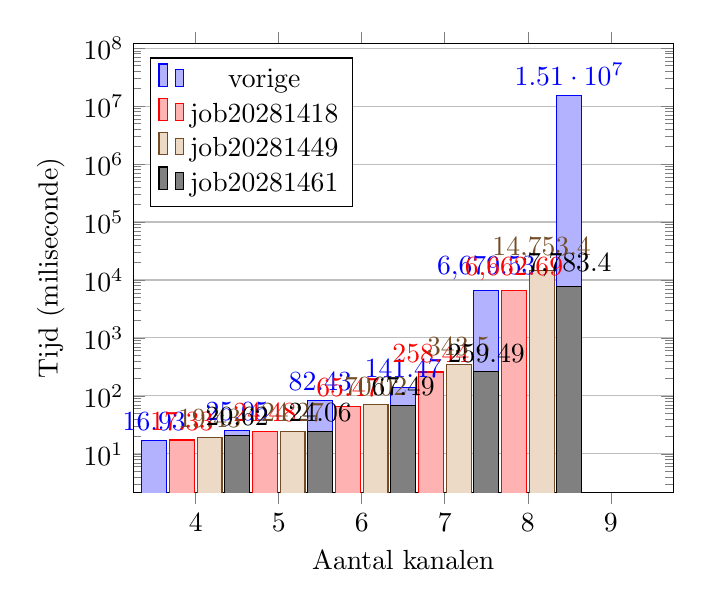
\begin{tikzpicture} 
	\begin{axis}[
		ylabel = Tijd (miliseconde),
		xlabel = Aantal kanalen,
		enlargelimits=0.15,
		ybar=1pt,
		ymode = log,
		log basis y = 10,
		bar width=9pt,
		nodes near coords,
		point meta=10^y,
		ymajorgrids = true, 
		legend pos = north west
]
\addplot
    coordinates {(4, 16.93) 			(5, 25.05) 			(6, 82.44) 			(7, 141.48) 		(8, 6680.31) (9, 15135358.01)};
\addplot
    coordinates {(4, 17.328771)		(5, 24.478119) 	(6, 65.476245)	(7, 258.468456)	(8, 6663.352099)};
\addplot
    coordinates {(4, 19.435501)		(5, 24.276606) 	(6, 70.032632)	(7, 343.578030)	(8, 14755.053198)};
\addplot
    coordinates {(4, 20.619104)		(5, 24.064872) 	(6, 67.499158)	(7, 259.514450)	(8, 7785.144087)};

%\addplot
%	coordinates {(9, 1101480000)};
\legend{vorige, job20281418, job20281449, job20281461};
\end{axis}

\end{tikzpicture}

\section{Conclusies}
Conclusie\cite{sortingNetworksSize2014}\\
Conclusie van wat er bereikt is en hoe er verder aan gewerkt kan worden.\cite{sortingNetworksTheEndGame}

\section*{Erkenning}
Hier komt de erkenning.




\bibliographystyle{named}
\bibliography{SortingNetworks}

\end{document}

